
\label{ch:Implémentations aristiques}

\section{Introduction}

Cette section conclut un point de vue artistique sur les aspects abordés dans les chapitres précédents. À partir de la transformation de Fourier en vocodeur de phase et en passant au morphing par des interprétations artistiques des patchs techniques mis en œuvre.

L'objectif de ce chapitre est de soutenir l'idée que l'analyse et la re-synthèse spectrales, et donc en expansion, le développement du signal musical  sont utiles aux scientifiques et aux artistes. En effet, les détails techniques antérieurs sont utilisés à des fins artistiques et esthétiques. Les exemples suivants consistent en une expérimentation personnelle et une interprétation du matériel technique déjà présenté.

\section{Le vocodeur de phase - \textit{Une capacité sans fin}}

\subsection{Super Phase Vocoder}

Dans le but de combiner plusieurs techniques du vocodeur de phase, nous avons implémenté un \guillemotleft \textit{super} vocodeur de phase\guillemotright . Cet outil spectral comprend l'étirement temporel, le freeze temporel, le décalage de hauteur, le morphing et d'autres effets bénéficiant de la fonction élémentaire du vocodeur de phase.

Le graphe \ref{FirstMorphingTry} presente le patch de contrôle de tous les paramètres du vocodeur de phase. Cette version du vocodeur de phase contient tous les effets étudiés dans les sections précédentes. Il n'y a pas quelque chose de particulièrement différent du vocodeur de phase de base pour le morphing apart quelques fonctionnalités de plus. Il est naturel de rechercher une fonctionnalité plus large pour le même outil. En suivant cette raisonement, nous avons implémenté tous les effets de base dans un seul patch. Les maths ici ne sont pas intéressants à analyser car ils ont tous été vus auparavant. Les détails les plus cruciaux se trouvent dans la séquence de tous les effets visibles dans figure \ref{SuperPhaseVoc}.

Dans le patch principal, vous pouvez voir deux pianos virtuels de contrôle permettant de modifier la hauteur de chaque son séparément. Idéalement, ce système devrait être automatique. Il faut estimer la fréquence de chaque son et corriger à mi-chemin la hauteur du son pour qu'il en soit de même. Une correction de hauteur intervient avant tout effet de morphing et n'affecte donc pas le résultat. Dans le patch principal, nous pouvons également trouver des commandes permettant de manipuler le filtre de Gabor, en ajustant les composantes de bruit de la phase qui, dans ce patch, sont identiques pour les deux sons. On peut également trouver des facteurs d’interpolation de magnitude et de phase pour le morphing, ainsi que la factorisation de la courbe, comme indiqué dans la section précédente. La dernière modification présentée dans ce patch est l'effet de \textit{freeze} qui contient les valeurs spectrales d'une seule fenêtre. Pour cet effet, deux types de filtrage sont également ajoutés pour modifier le timbre des spectres gelés.


\begin{figure}
\centering
\begin{subfigure}{\textwidth}
  \centering
  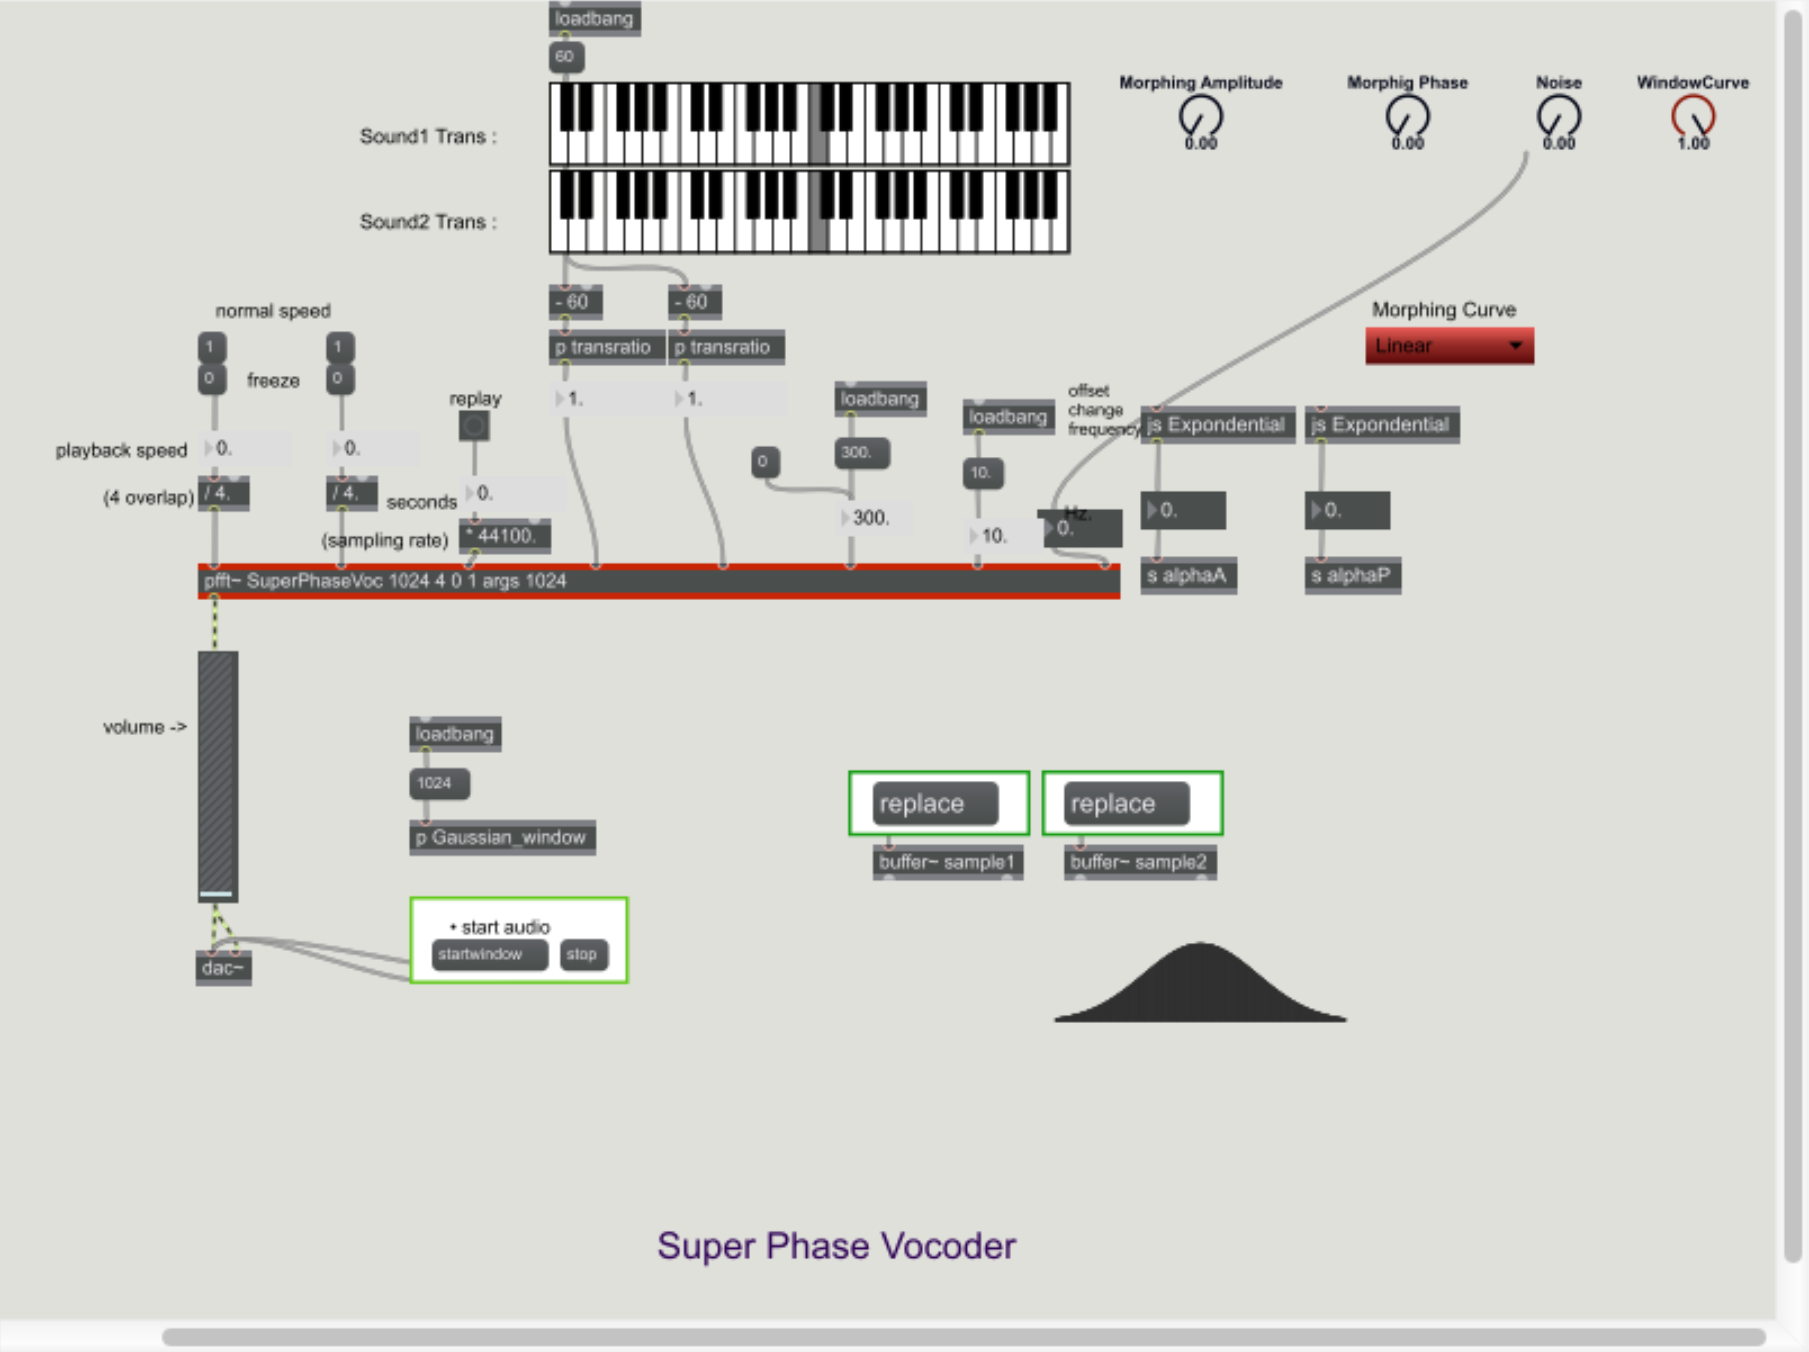
\includegraphics[width=.8\linewidth]{Graphs/FirstMorphingTry.png}
  \caption{Super Phase Vocoder I}
  \label{FirstMorphingTry}
\end{subfigure}

\begin{subfigure}{\textwidth}
  \centering
  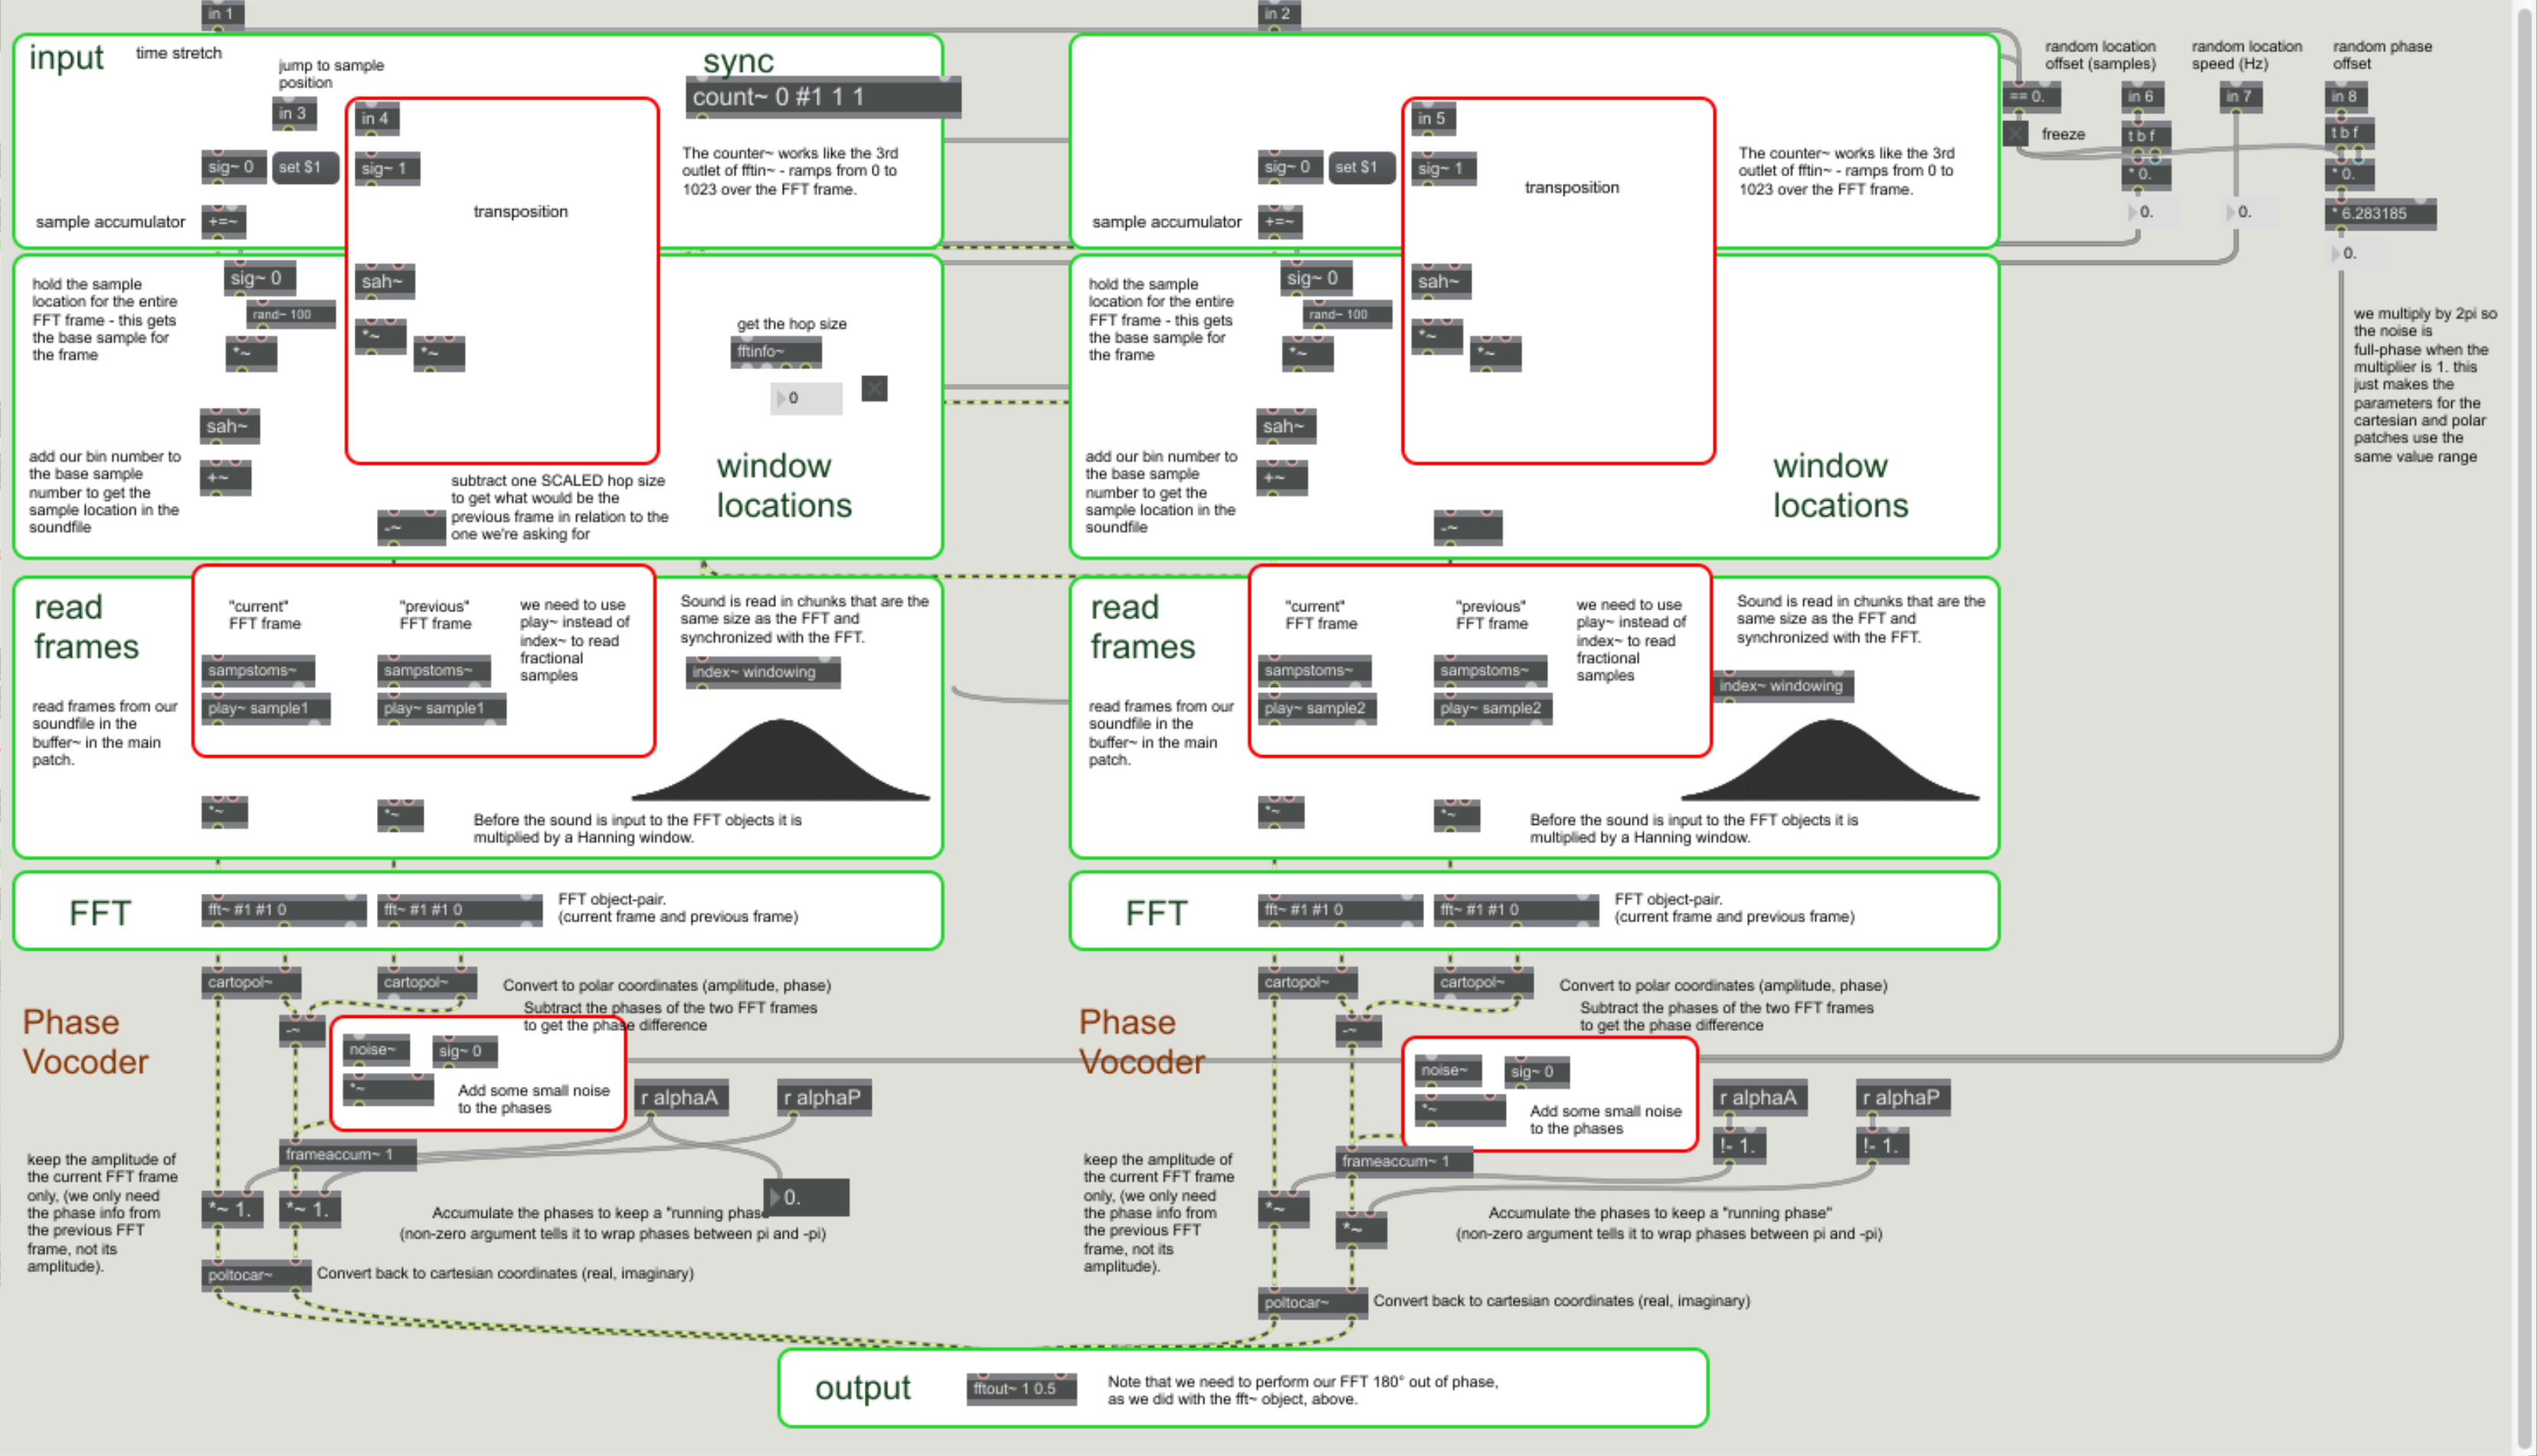
\includegraphics[width=.8\linewidth]{Graphs/SuperPhaseVoc.png}
  \caption{Super Phase Vocoder II}
  \label{SuperPhaseVoc}
\end{subfigure}
\caption{Super Phase Vocoder}
\label{PhaseVocoder}
\end{figure}

\subsection{Phase interference}
    Dans ce patch MaxMSP, nous étudions une modification des coordonnées polaires après l’étape de l’analyse. Nous ajoutons simplement un oscillateur de phaseur après la FFT et l’appliquons à chaque amplitude et phase corrigée de la fenêtre. De cette façon, l'identité du signal n'est pas modifiée, mais une fréquence oscillante interfère avec chaque index de la fenêtre FFT. La formule de cette modification est présentée ci-dessous par l'équation de synthèse.

\begin{figure}
  \centering
  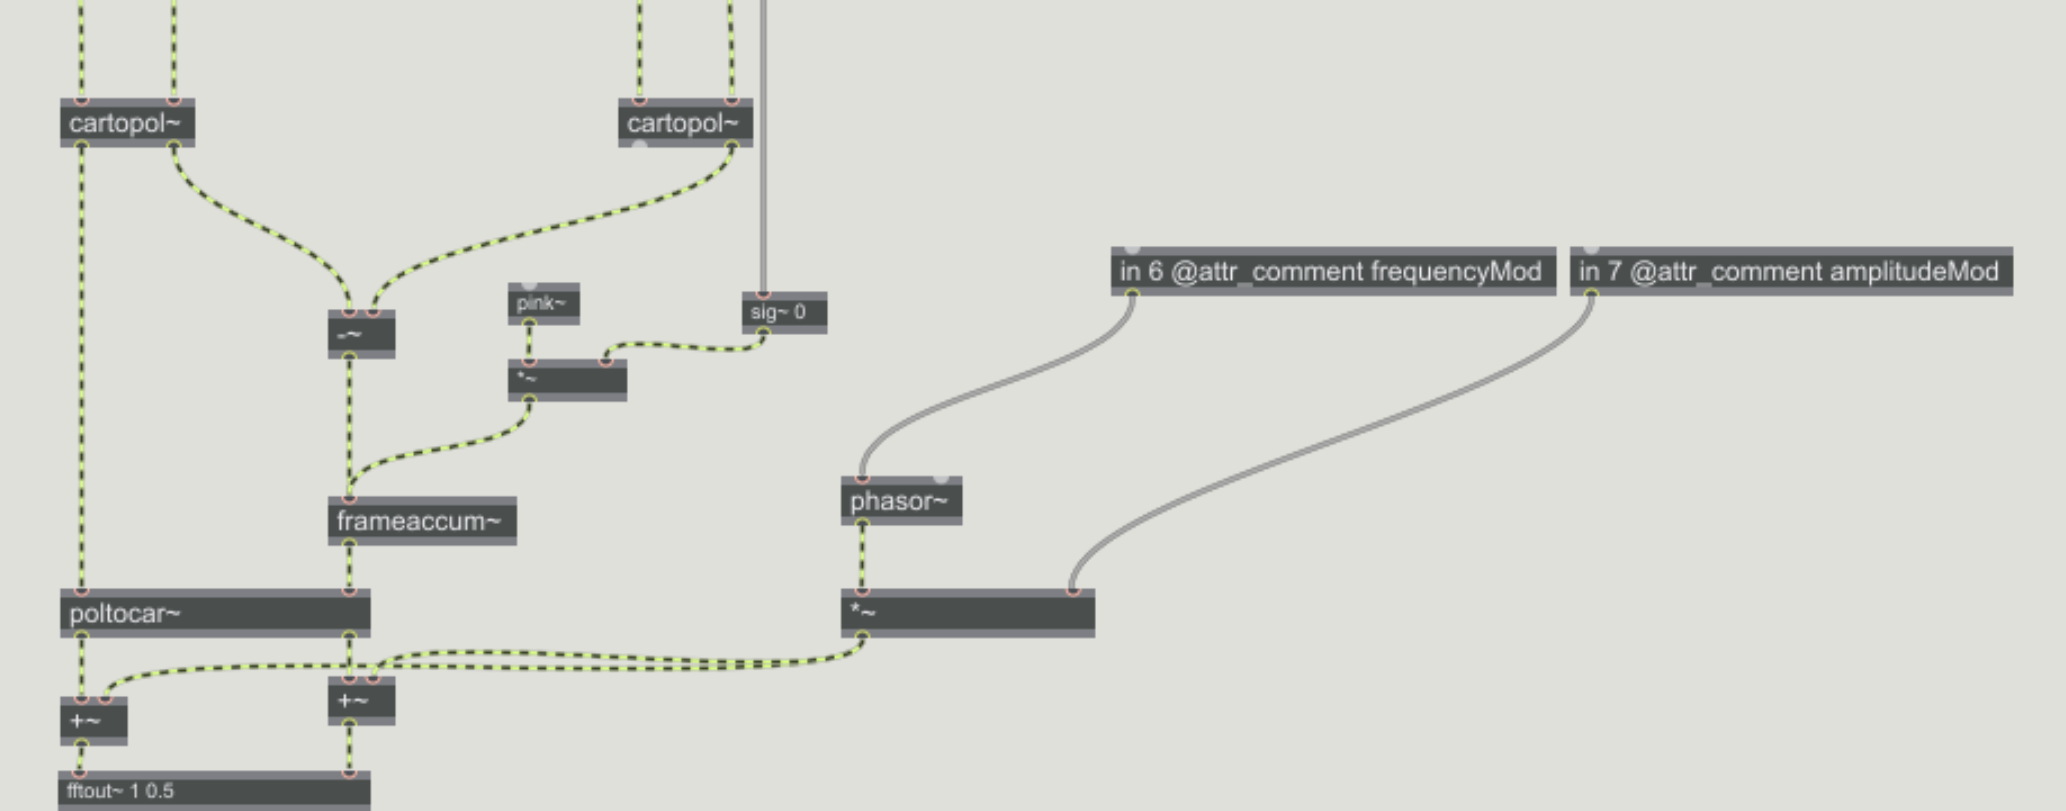
\includegraphics[width= 0.5 \textwidth]{Graphs/phasorInt.png}
  \caption{modulation \\ des coordonées polaires}
  \label{phasorInt}
\end{figure}

    \begin{equation}
      y(n, k) = \sum_{k=1}^K (A[n]+phi(n)) \; e^{j (\theta_k(n) +\phi(n)}
    \end{equation}
    
    Où $y (n, k)$ est le signal fenêtré après l'analyse. K est le nombre de sinisoides, $ A [n] $ est la magnitude instantanée, $ \theta $ est la phase instantanée et $ \phi (n) $ est le phaseur instantané donné par la formule:

    \begin{equation*}
        \phi(n) = n - floor(n)
    \end{equation*}

    Nous pouvons voir que le modèle sous-jacent de la FFT est utilisé pour représenter cette modification. D'autres modèles pourraient parfaitement décrire cet effet, mais dans cette version, il est plus direct. Dans la figure correspondante \ref{phasorInt}, nous pouvons voir le phaseur moduler la magnitude et la phase. La fréquence et l'amplitude du phaseur sont contrôlées dans le patch principal contenant l'objet pfft $ \thicksim $.

\subsection{Modulation au bruit}

\begin{wrapfigure}{r}{0.5\textwidth}
  \vspace{-20pt}
  \begin{center}
    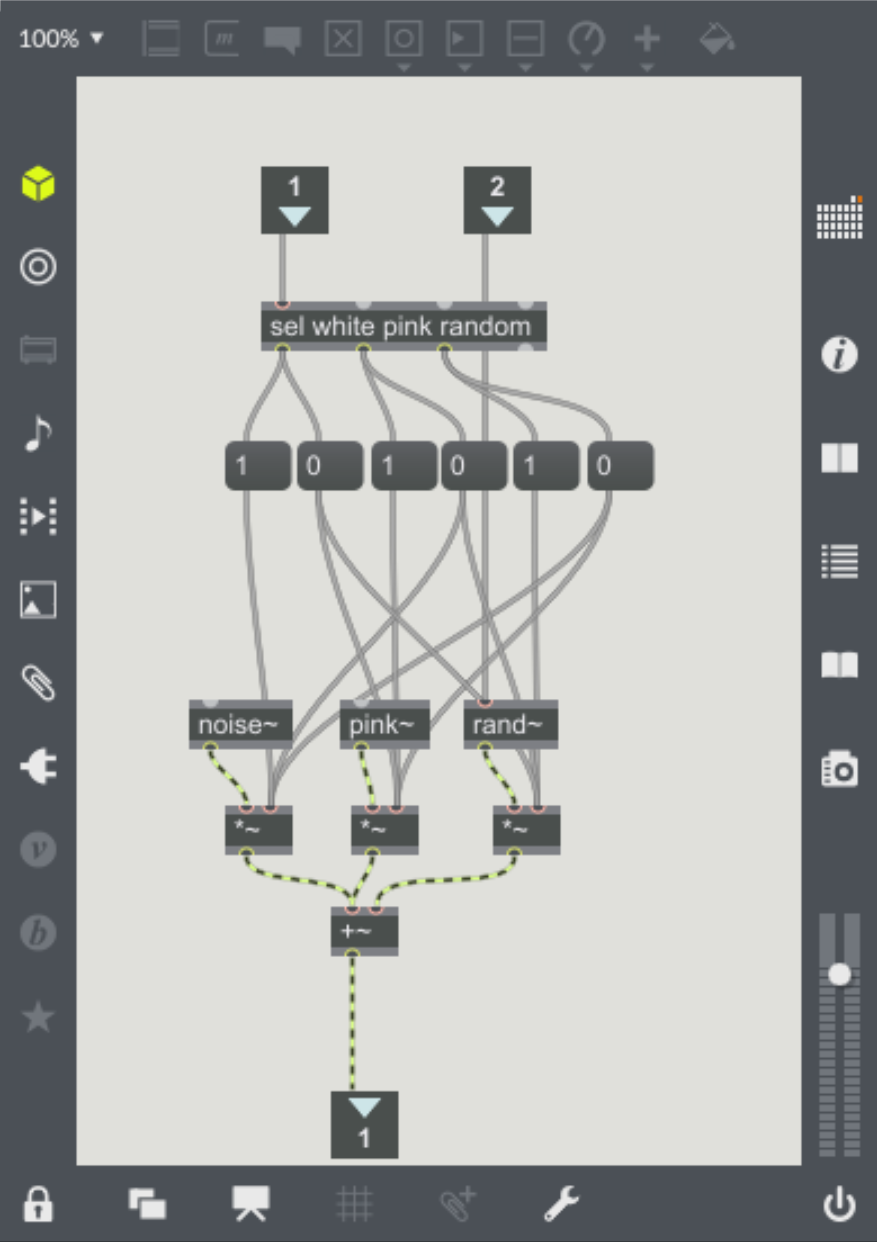
\includegraphics[width=0.48\textwidth]{Graphs/Noise_Select.png}
  \end{center}
  \vspace{-20pt}
  \caption{Selection du bruit}
  \vspace{-10pt}
\end{wrapfigure}

    Dans ce vocodeur de phase, nous étudions une modulation de bruit sur la composante de fréquence. Nous avons ajouté la composante de bruit et essayé différents générateurs de bruit tels que $ rand \thicksim $, pink-noise, white-noise et en même temps nous avons contrôlé le facteur d'amplitude de cette composante. Le sous-patch pour la sélection du bruit est visible dans la figure \ref{Noise_Select}. Un objet umenu fonctionne comme un stade de sélection pour l'utilisateur du maître transmettant ses valeurs au sous-patch pfft.

    La phase corrigée, par la fenêtre FFT de chevauchement, est multipliée par le facteur du bruit. Dans les dossiers sonores de cette thèse, on entend les différentes modulations de bruit, mais le résultat sonore n’est pas évident. Le facteur de bruit est utilisé pour la naturalisation du son car les fréquences continues pures ne sont pas produites dans les sons réels. Par conséquent, une petite correction de l'oscillateur de bruit ne donne pas un résultat strictement différent.

\subsection{Filtre aletoire sur la position du buffer$\thicksim$}

    Dans ce patch, nous modulons la position du tampon via un générateur de signaux aléatoires qui transmet ses valeurs au lecteur de la position du fichier. Pour être plus précis, nous filtrons les harmoniques de la FFT en produisant des nombres aléatoires pour chaque harmonique et en ne calculant l'harmonique $ k-$\ième que si le nombre aléatoire correspondant est inférieur à sa valeur d'index.

\begin{wrapfigure}{r}{0.5\textwidth}
  \vspace{-20pt}
  \begin{center}
    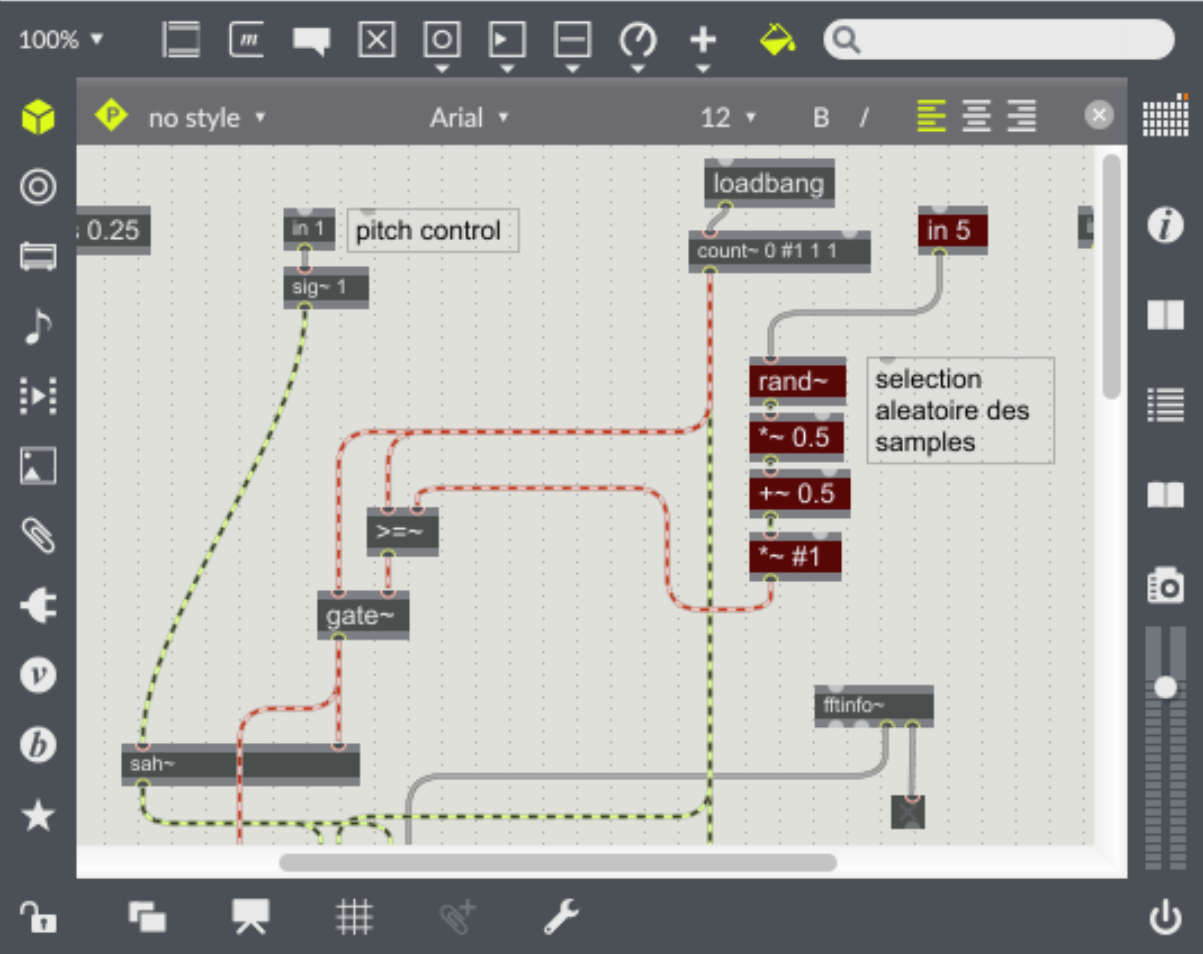
\includegraphics[width=0.48\textwidth]{Graphs/random_sampling.png}
  \end{center}
  \vspace{-20pt}
  \caption{Filtre aletoire}
  \vspace{-10pt}
\end{wrapfigure}

    Le générateur aléatoire est créé par l'objet $ random \thicksim $ avec un filtre modulant la fréquence de la génération de valeur aléatoire. La valeur transmise au lecteur de l'objet $ play \thicksim $ est modulée par un détenteur d'échantillon qui prend en entrée la sortie d'un compteur et la valeur générée de manière aléatoire. Le porte-échantillon est créé manuellement par un objet supérieur à un objet et une porte. De cette manière, nous conservons et publions de manière abstraite des valeurs dans la fenêtre FFT, créant ainsi un système hybride de modulation de la hauteur et de la lecture. La modulation peut être trouvée dans la figure.
    

\section{Morphing visuel}

En avançant sur le morphing visuel, nous avons implémenté le patch suivant avec l’aide du Jitter, pour une interpolation linéaire entre deux dessins.

    \begin{figure}
        \centering
        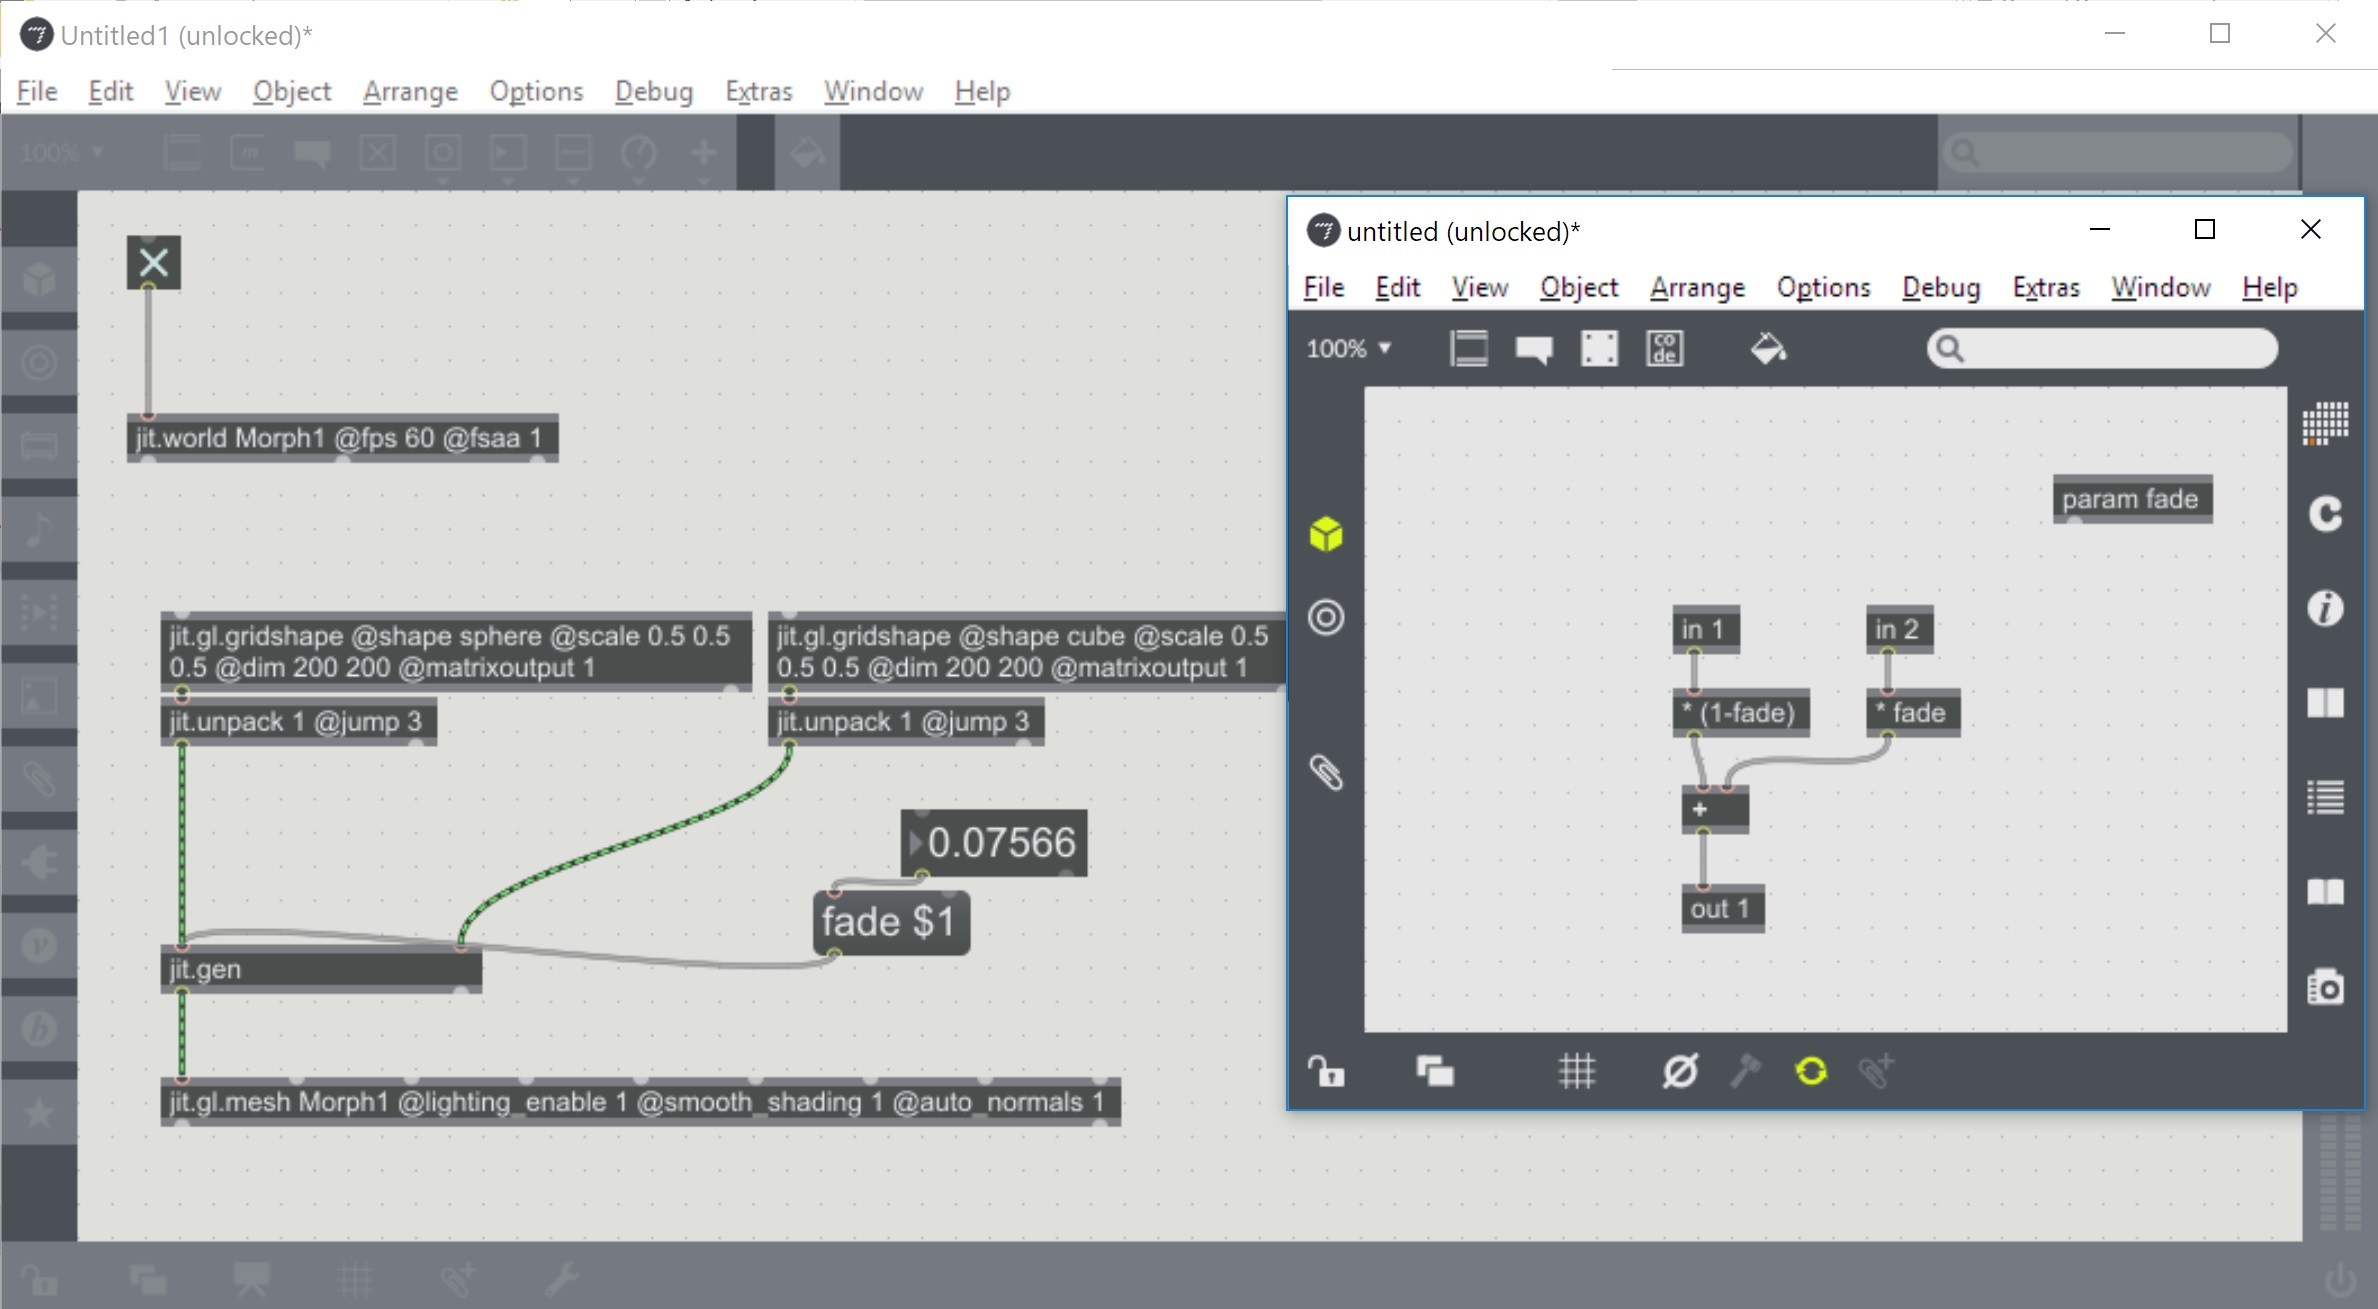
\includegraphics[width = \textwidth ]{Graphs/Morphing_patch.jpg}
        \caption{Visual Morphing}
        \label{VisualMorph}
    \end{figure}


En répétant la formule de base de morphing $M(\alpha) = \alpha\widehat {S_1} + [1 -\alpha]\widehat {S_2} $ une patch sur le morphing en 3D était implémenté avec l'aide de l'objet jit.gen (figure \ref{VisualMorph}).

Donc, fondamentalement, un morphing visuel est facile à faire avec les fonctions 3D primordiaux de Jitter telles que jit.gl.gridshape et jit.gen pour une personnalisation de la procédure de morphing. L'objet jit.gl.mesh est utilisé pour combiner le résultat du morphing alors que l'objet gen est contrôlé par un facteur de fondu.

À l'intérieur de gen, une procédure assez simple se produit. Les données multidimensionnelles provenant des matrices de localisation sont utilisées séparément pour chaque forme et leur amplitude est multipliée par le facteur $\alpha$ comme dans le morphing audio.

Bien entendu, nous pourrions également implémenter le script expondential.js pour une courbe de morphing différente sur le visuel.

Dans le patch suivant nous sommes allés un etape plus loin en separent tout composant d'un modèle tri-dimensionel dans jitter. Nous distinguons les valeurs des matrices, des normals et de la texture. Nous avons ajoutés egalement une interpolation du couleur. Le patch est en disposition en figure \ref{VisualMorph2}.

    \begin{figure}
        \centering
        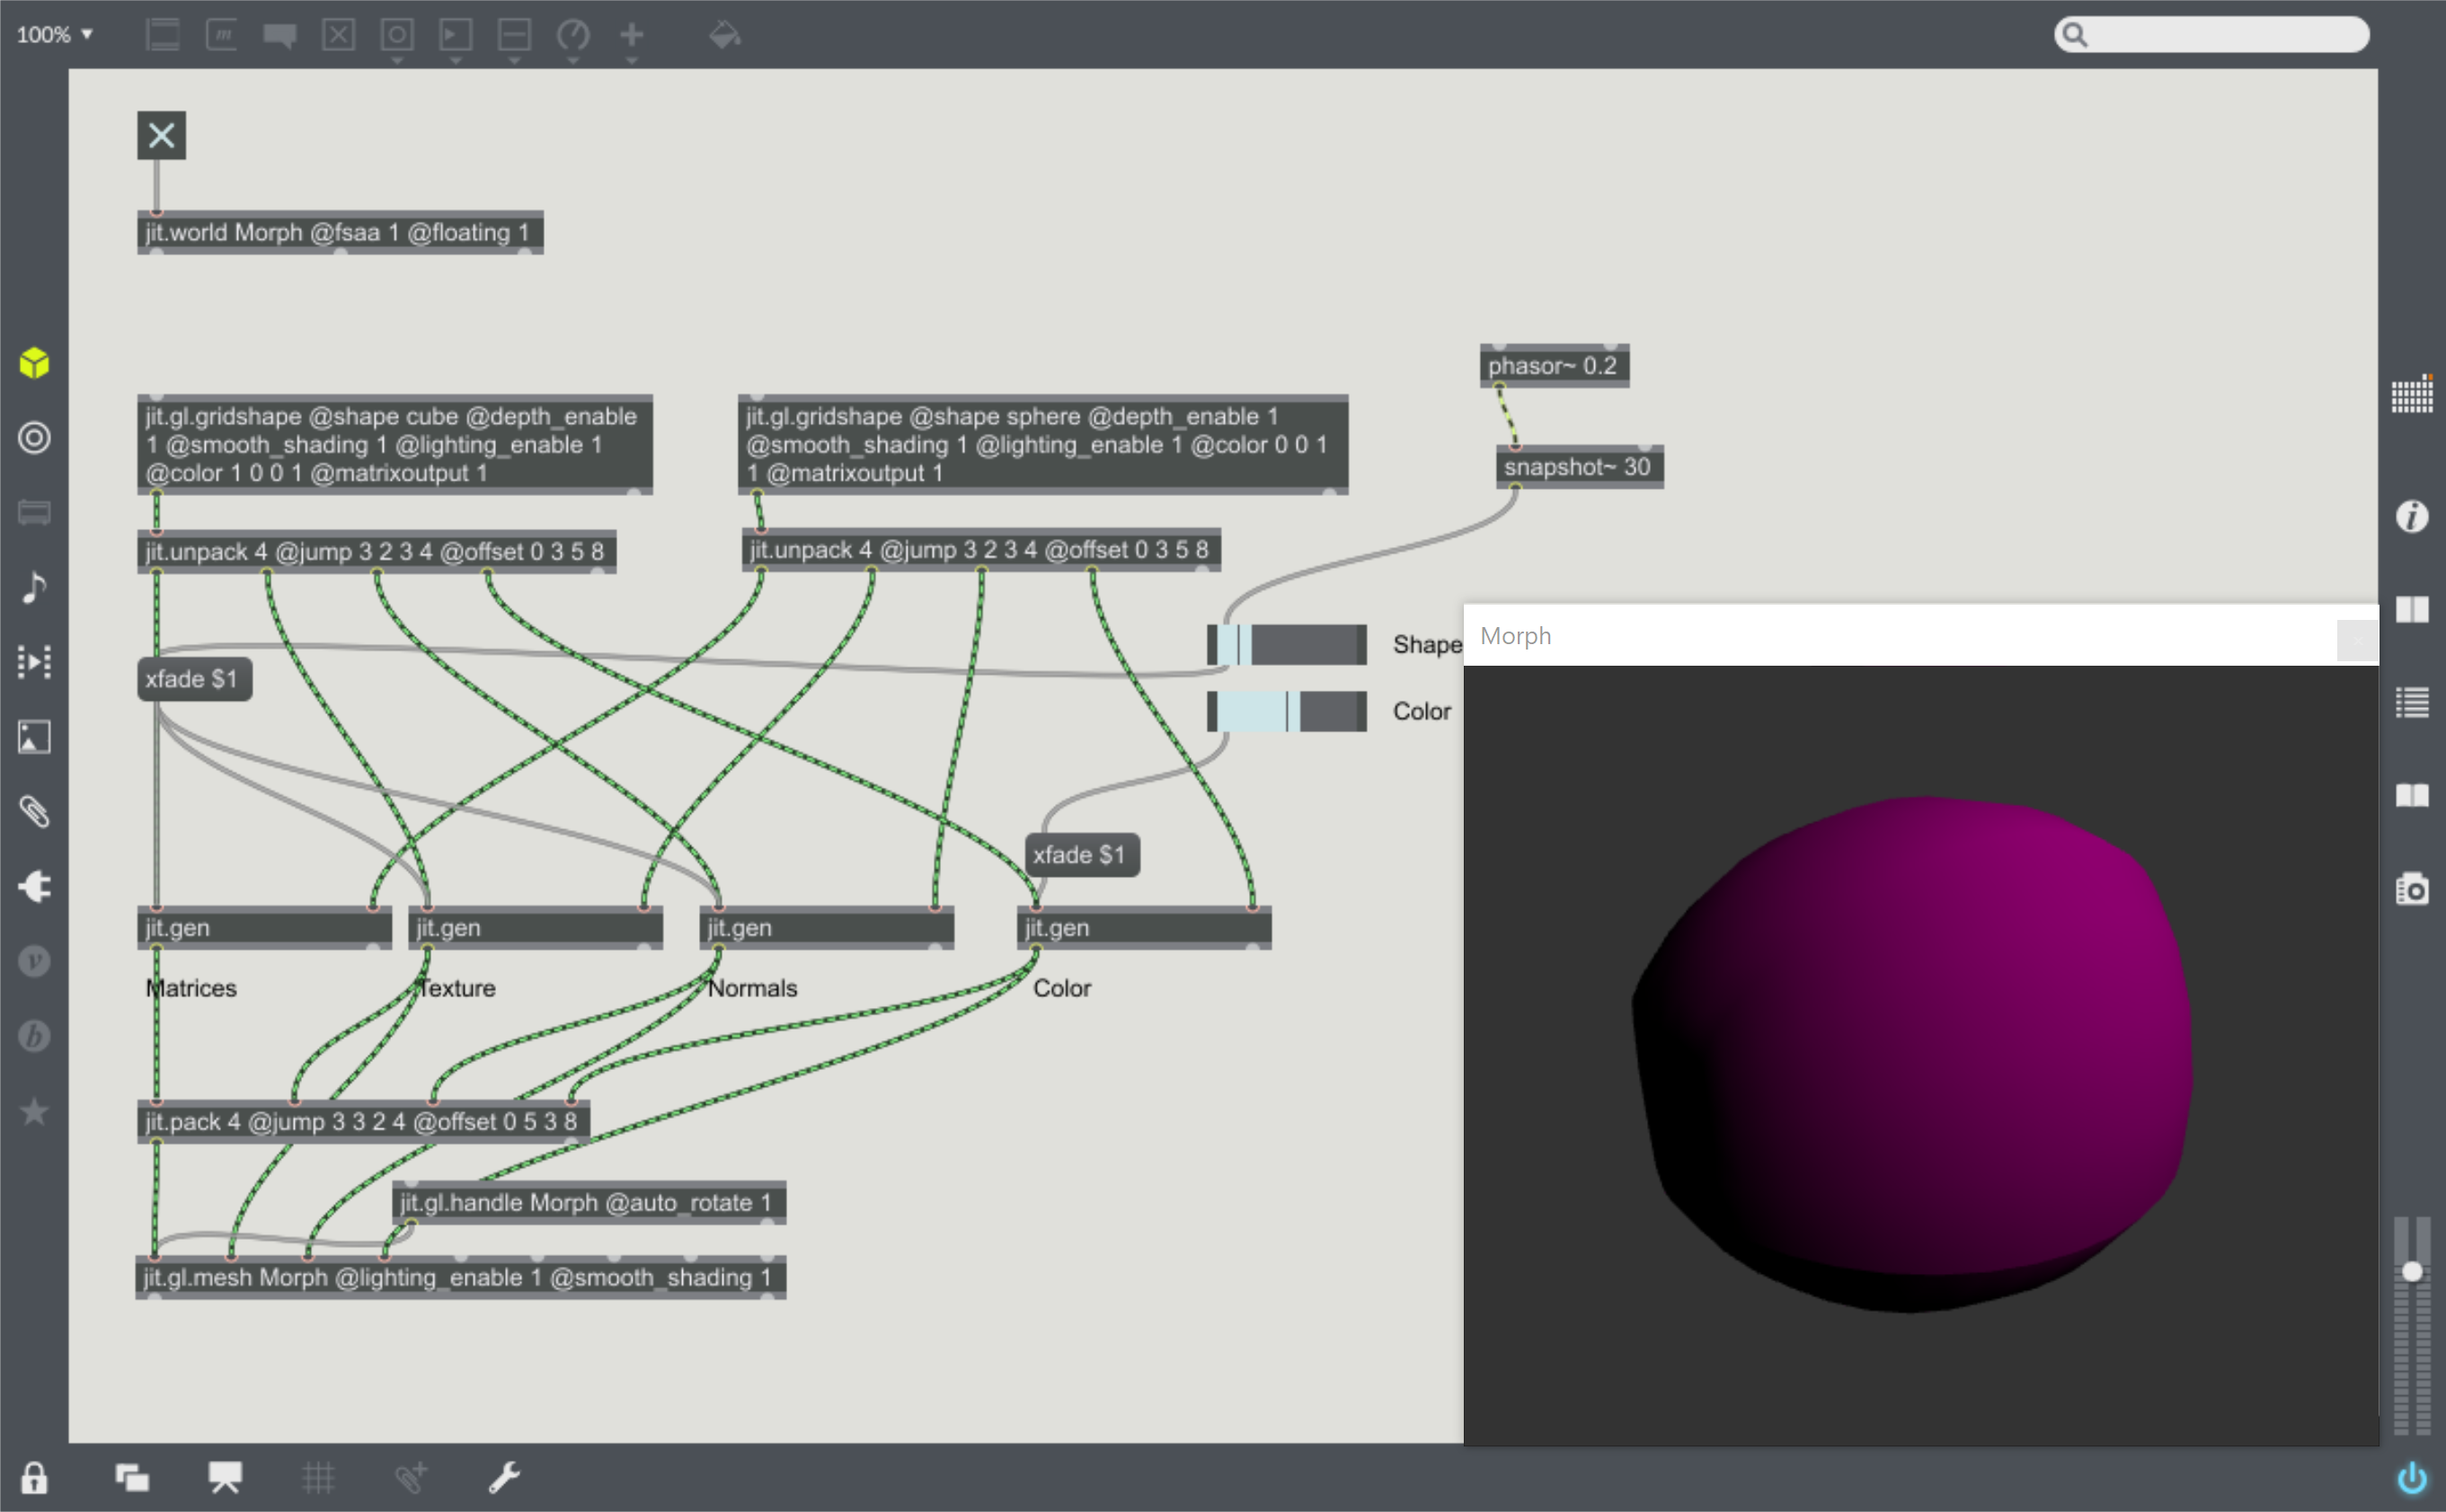
\includegraphics[width = \textwidth ]{Graphs/ShapeMorphing1.png}
        \caption{Visual Morphing $2^{ème}$ version}
        \label{VisualMorph2}
    \end{figure} 

\begin{figure}
\begin{subfigure}{.5\textwidth}
  \centering
  \caption{Interpolation de la forme : $0.0$ \\ Interpolation couleur : $0.0$}
  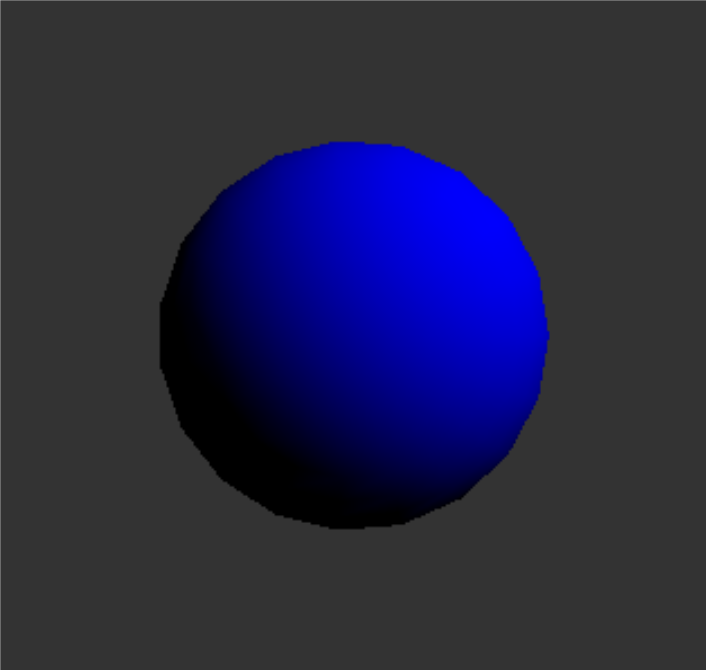
\includegraphics[width=1\linewidth]{Graphs/morph1.png}  
  \label{fig:sub-first}
\end{subfigure}
\begin{subfigure}{.5\textwidth}
  \centering
  \caption{Interpolation de la forme : $0.4$ \\ Interpolation couleur : $0.8$}
  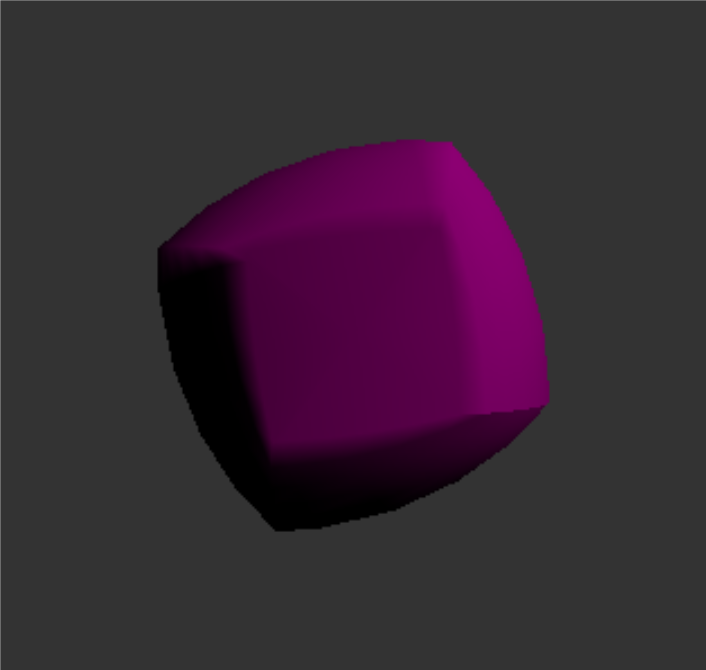
\includegraphics[width=1\linewidth]{Graphs/morph2.png}  
  \label{fig:sub-second}
\end{subfigure}

\begin{subfigure}{.5\textwidth}
  \centering
  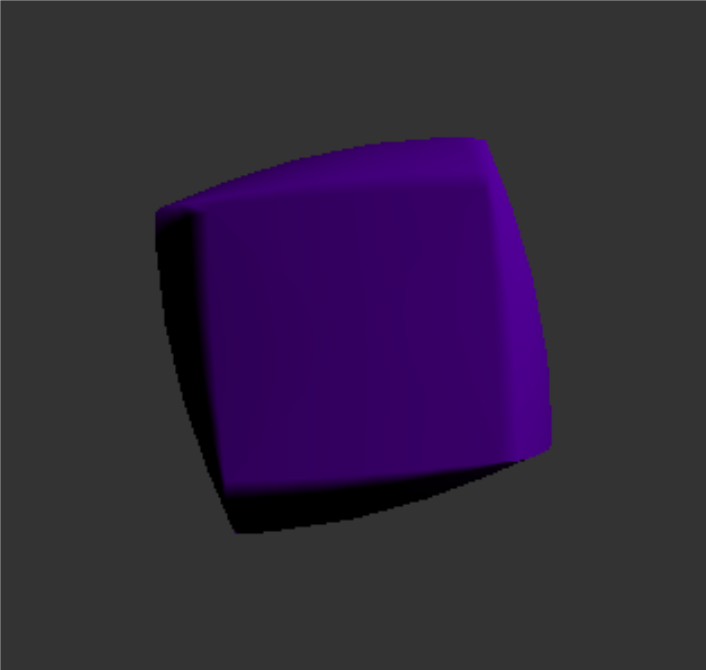
\includegraphics[width=1\linewidth]{Graphs/morph3.png}  
  \caption{Interpolation de la forme : $0.8$ \\ Interpolation couleur : $0.4$}
  \label{fig:sub-third}
\end{subfigure}
\begin{subfigure}{.5\textwidth}
  \centering
  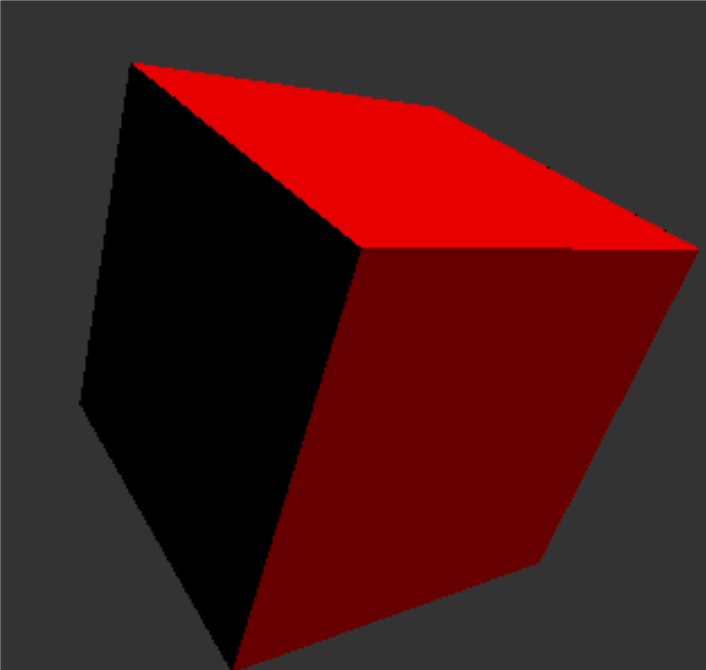
\includegraphics[width=1\linewidth]{Graphs/morph4.png}  
  \caption{Interpolation de la forme : $1.0$ \\ Interpolation couleur : $1.0$}
  \label{fig:sub-fourth}
\end{subfigure}
\caption{Stades du morphing visuel}
\label{fig:fig}
\end{figure}

\subsection{Visualization du spectre}
    
    Dans ce patch, beaucoup de travail sur la gigue a été implémenté avec un vocodeur de phase. Ce code permet de visualiser les informations spectrales d’un son sous la forme d’un paquet de lignes bidimensionnelles imitant les harmoniques trouvées lors d’une analyse de Fourier.

    Ce patch utilisé à l'unisson avec un vocodeur de phase pour le morphing ou même le simple décalage de pitch permet de visualiser l'évolution du spectre dans un environnement de rendu en temps réel. Dans ce code, nous utilisons une bibliothèque de gigue supplémentaire pour produire plusieurs objets de gigue rendus dans un espace tridimensionnel virtuel. L'objectif de cette thèse n'étant pas orienté image, nous ne dévoilerons pas beaucoup d'informations sur le traitement.

    Nous allons attribuer ici brièvement les objets les plus emblématiques de la gigue utilisés dans ce patch. L'objet \textit{jit.world} crée une nouvelle fenêtre et un espace de rendu virtuel tridimensionnel pouvant également contenir de la physique, des plans, des objets tridimensionnels, contrôler la position de la caméra, la couleur d'arrière-plan, etc. Le \textit{jit.gridshape} rend un objet tridimensionnel dans une fenêtre. La bibliothèque \textit{jit.mo} réplique de manière fluide les copies d’objets de gigue. Et le \textit{jit.catch} prend un signal et le traduit en matrice de gigue pour la visualisation potentielle.

    Pour transformer les informations spectrales en données tridimensionnelles, nous utilisons bien sûr une transformation FFT et un tampon qui lit les composantes polaires de la FFT (magnitude et phase) avec un objet $ peek \thicksim $ les envoie dans un tampon. Un objet $ lookup \thicksim $ récupère le contenu du tampon et les entre dans l'objet \textit{jit.catch}.

    Nous pouvons régler la dimension de \textit{jit.mo} pour générer plus d'harmoniques. Le son de sortie du vocodeur est envoyé à ce patch de visualisation harmonique pour saisir le résultat dans un espace 3D.


    \begin{figure}
        \centering
        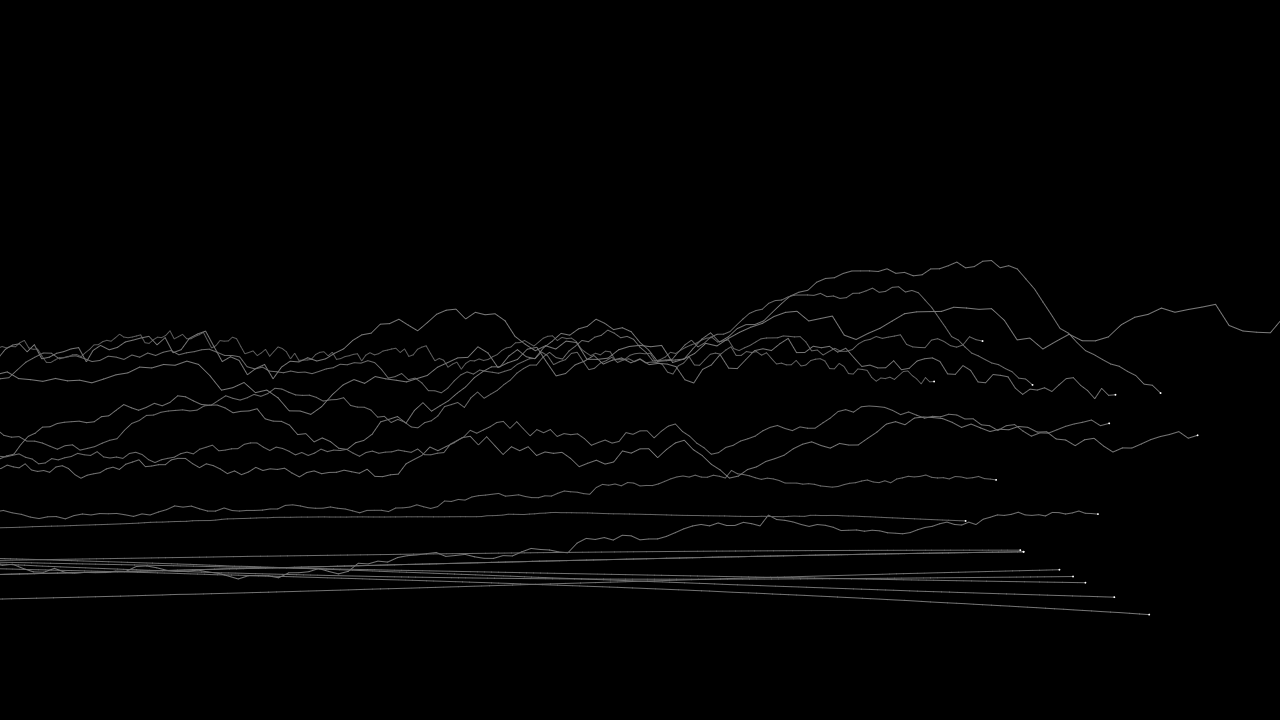
\includegraphics[width = \textwidth ]{Graphs/SpectralWindow.png}
        \caption{Harmoniques dans l'espace}
        \label{SpectralWindow}
    \end{figure} 

    \begin{figure}
        \centering
        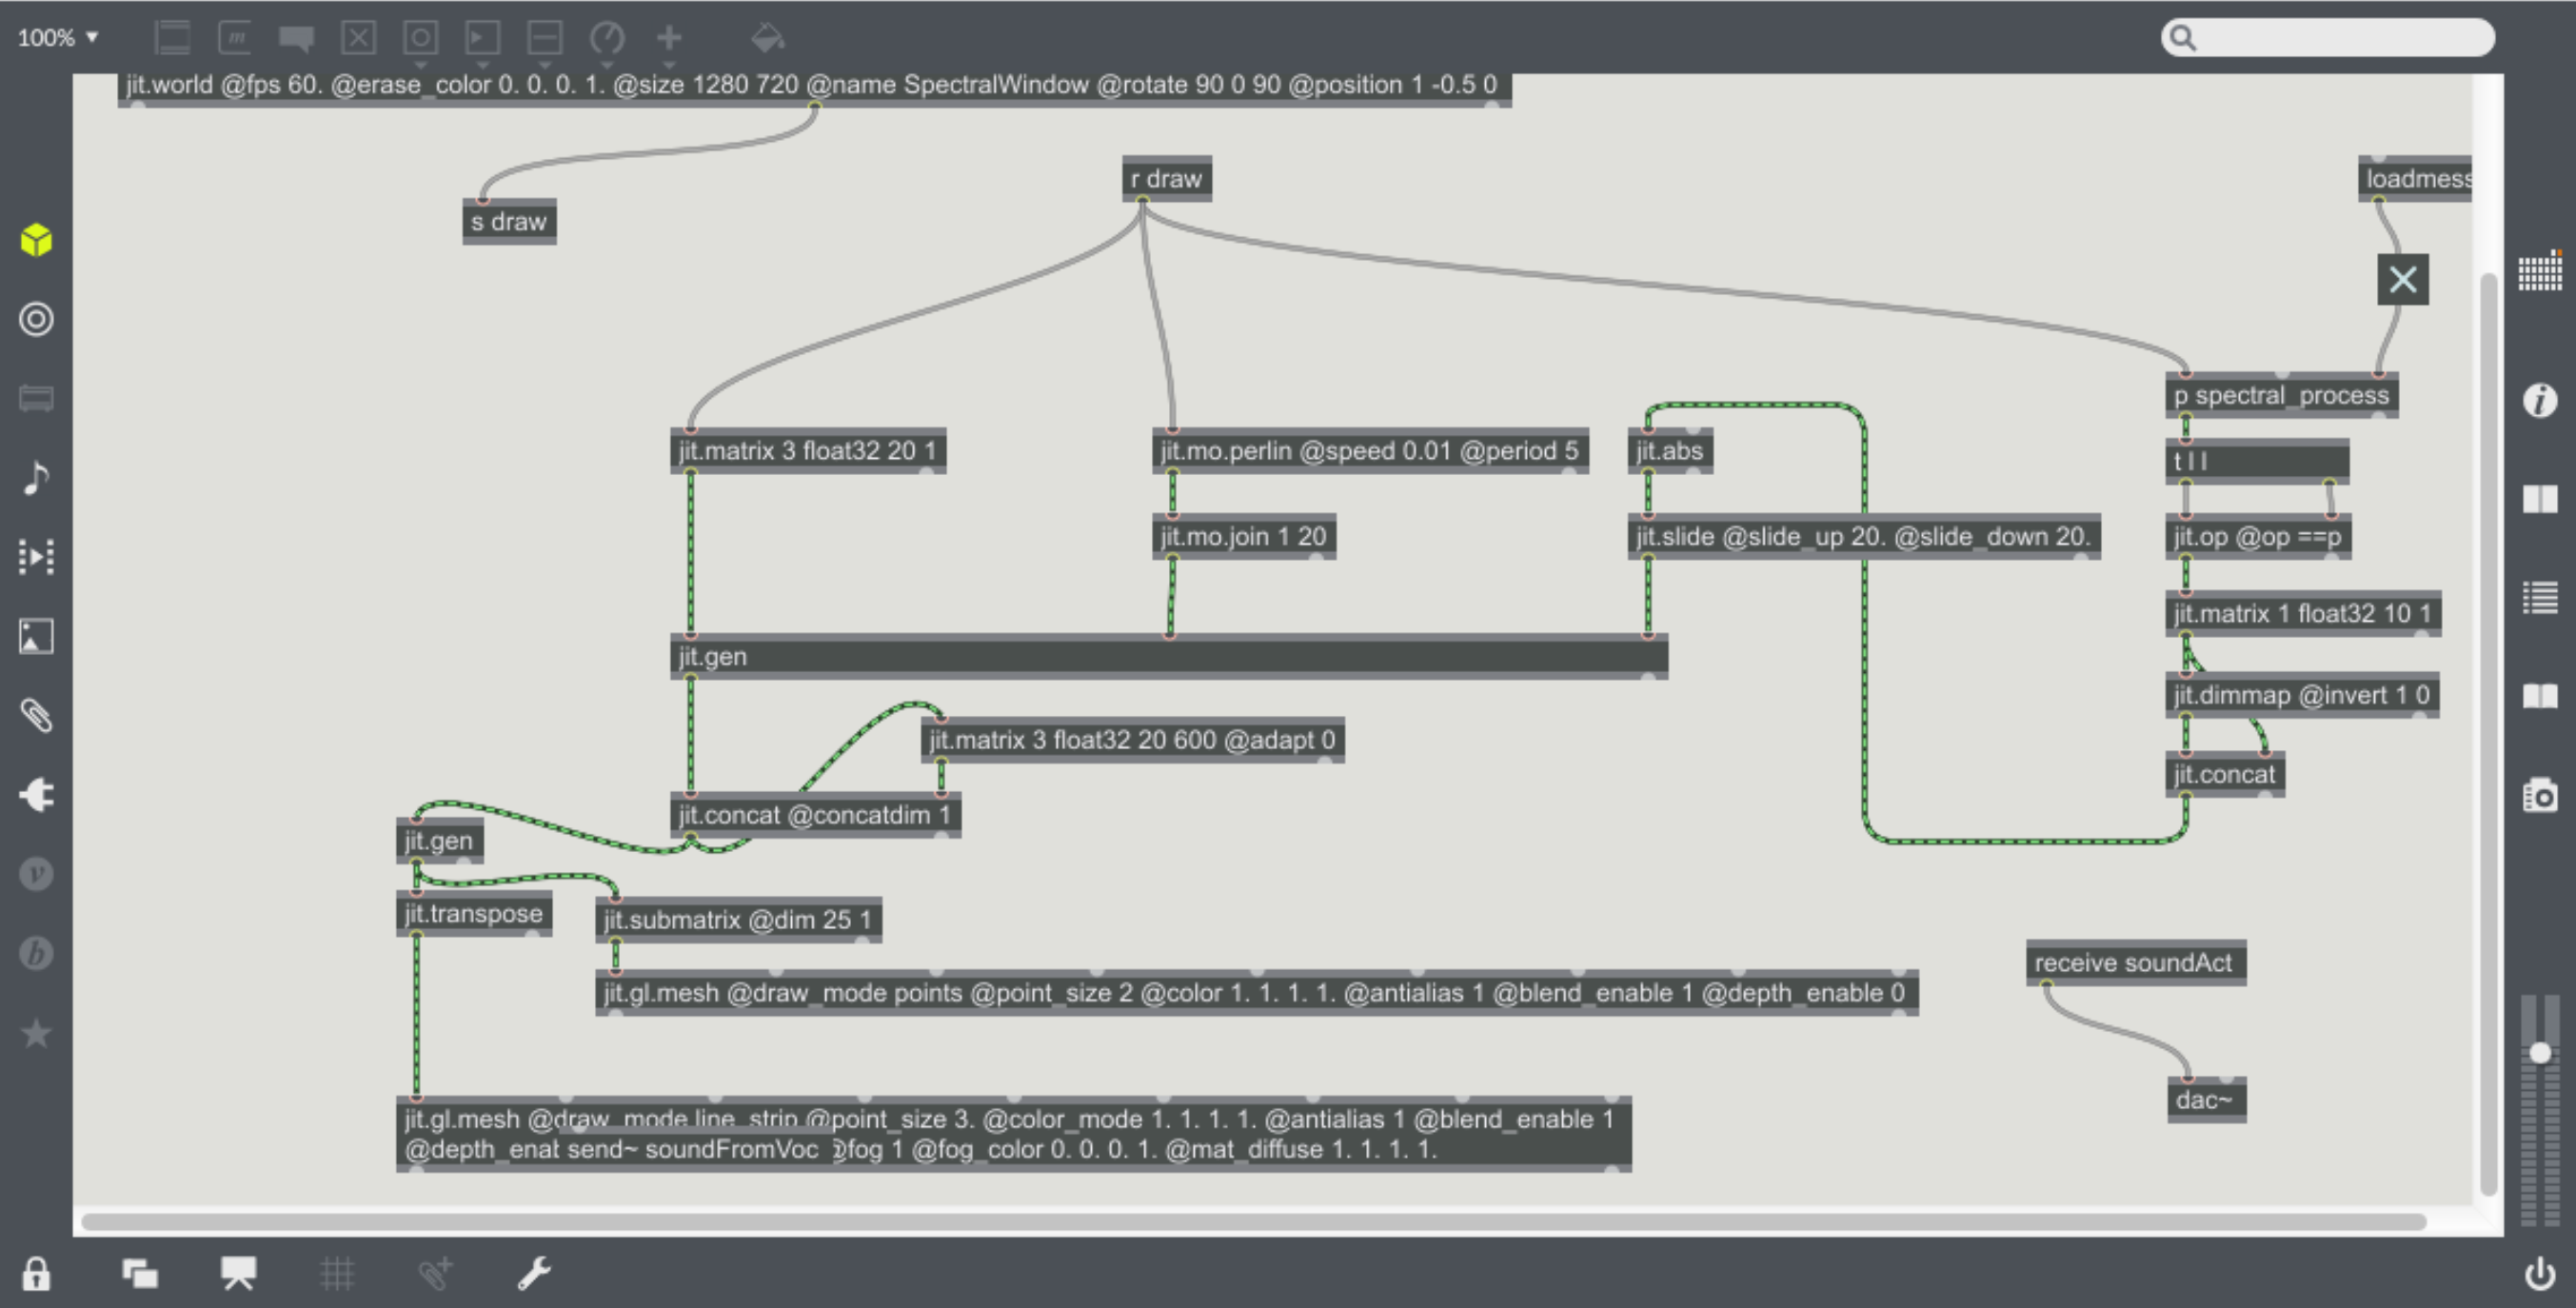
\includegraphics[width = \textwidth ]{Graphs/SpectralDraw.png}
        \caption{Le patch qui control les objets jitter}
        \label{SpectralDraw}
    \end{figure} 

